% This script will pull the tex-created pdfs of all specified classe notes together into one pdf container

\documentclass{report}
\usepackage{pdfpages}


% Note: there are two ways to pull LaTeX documents together.  This tex file simply combined pre-compiled pdfs.  The other is to pull together and compile the individual tex files together (which requires those files not having their own preamble setups).
% See https://tex.stackexchange.com/questions/155867/making-one-pdf-file-from-multiple-pdfs-or-tex

\title{\textbf{Analytical Workflows}\\All course notes strung together}

\begin{document}
	\maketitle

	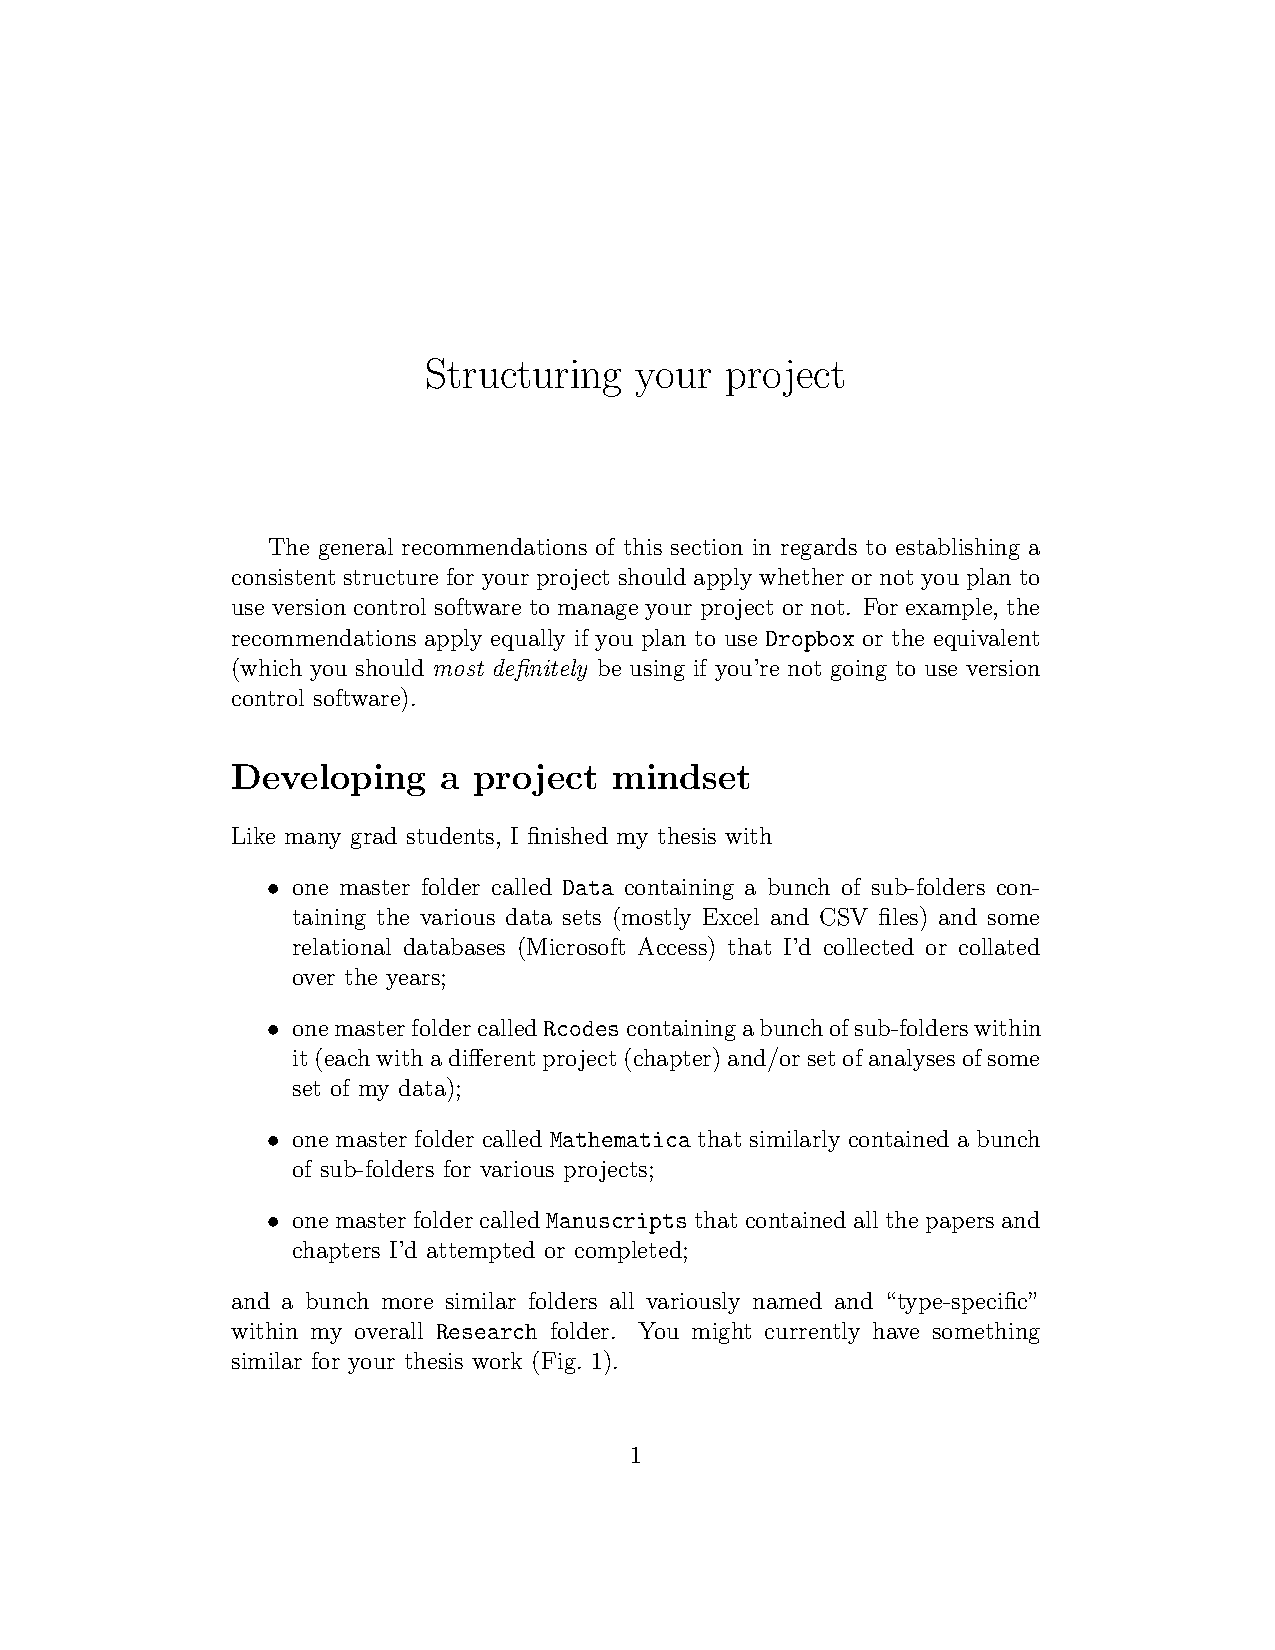
\includepdf[pages=-]{../../classes/StructuredProjects/tex/StructuredProjects.pdf}
	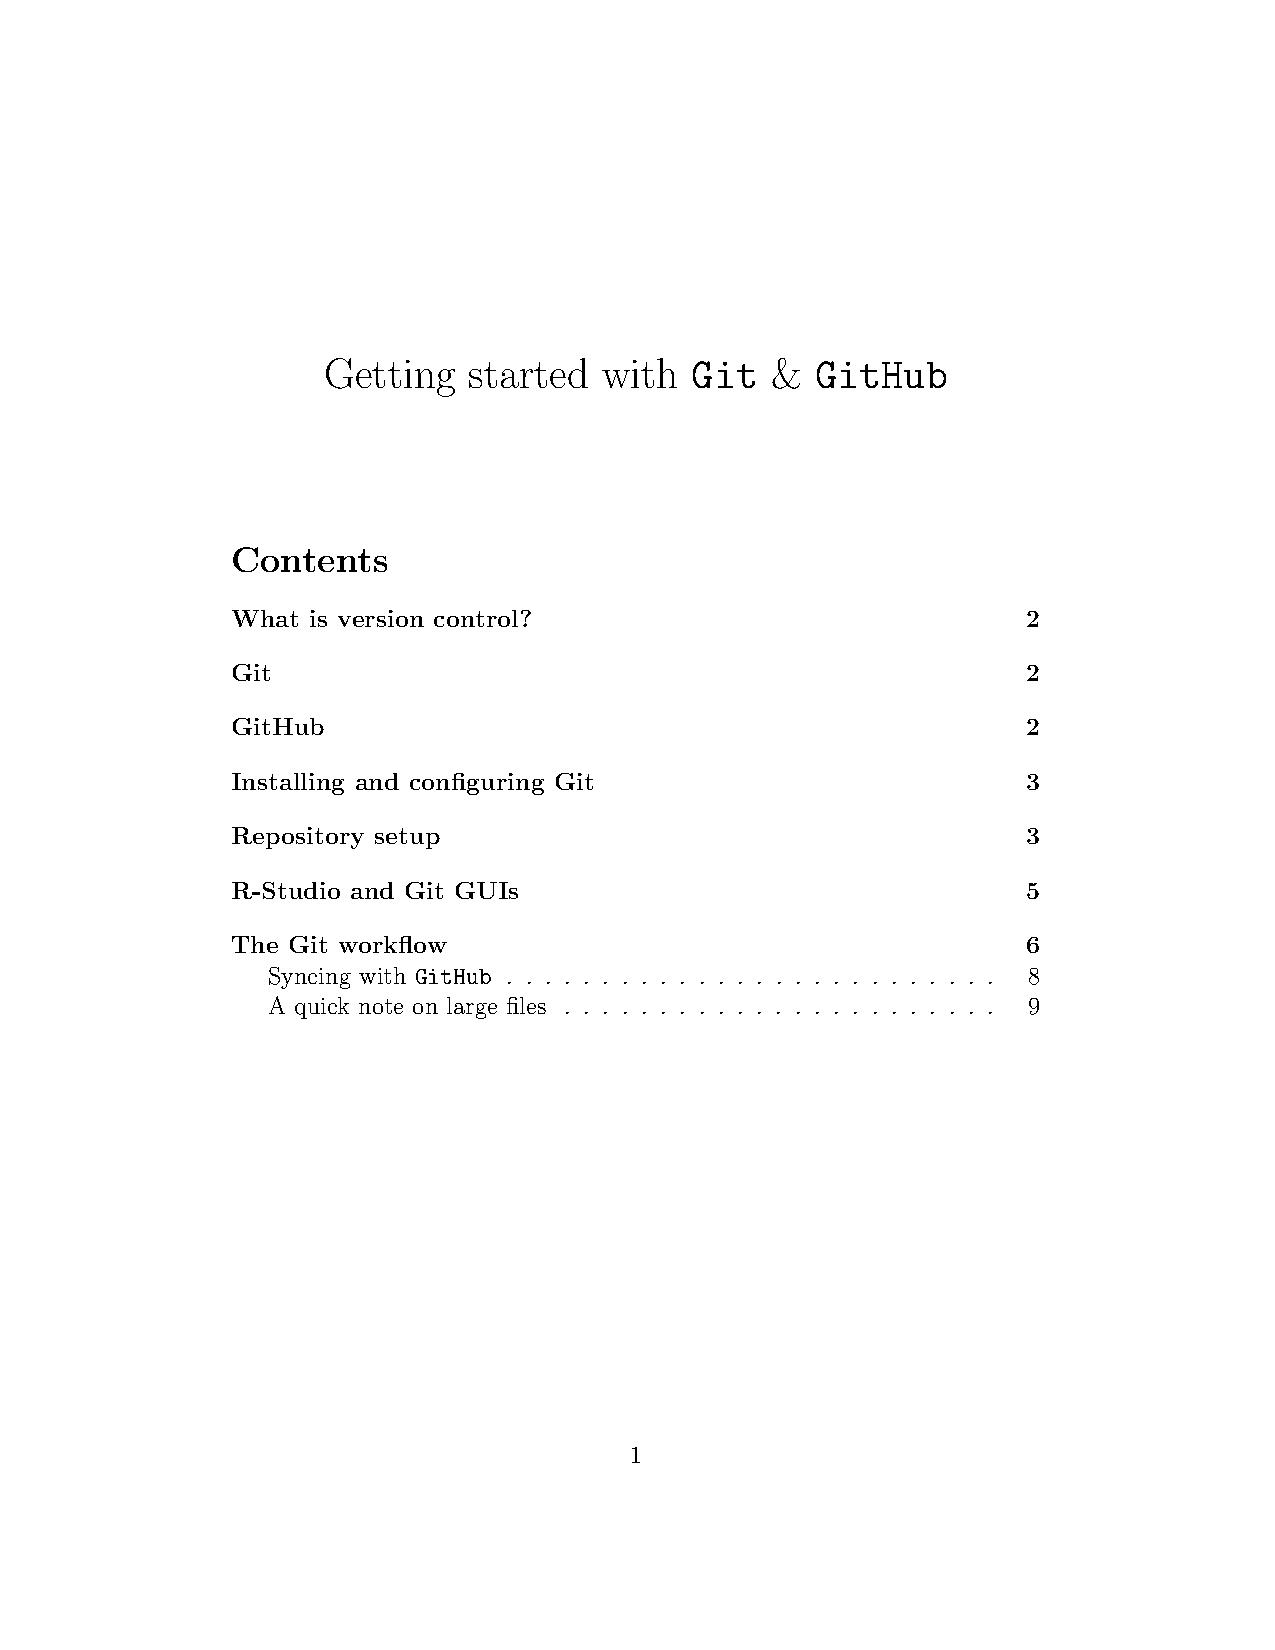
\includepdf[pages=-]{../../classes/VersionControl_Git_part_1/tex/Intro2Git}
	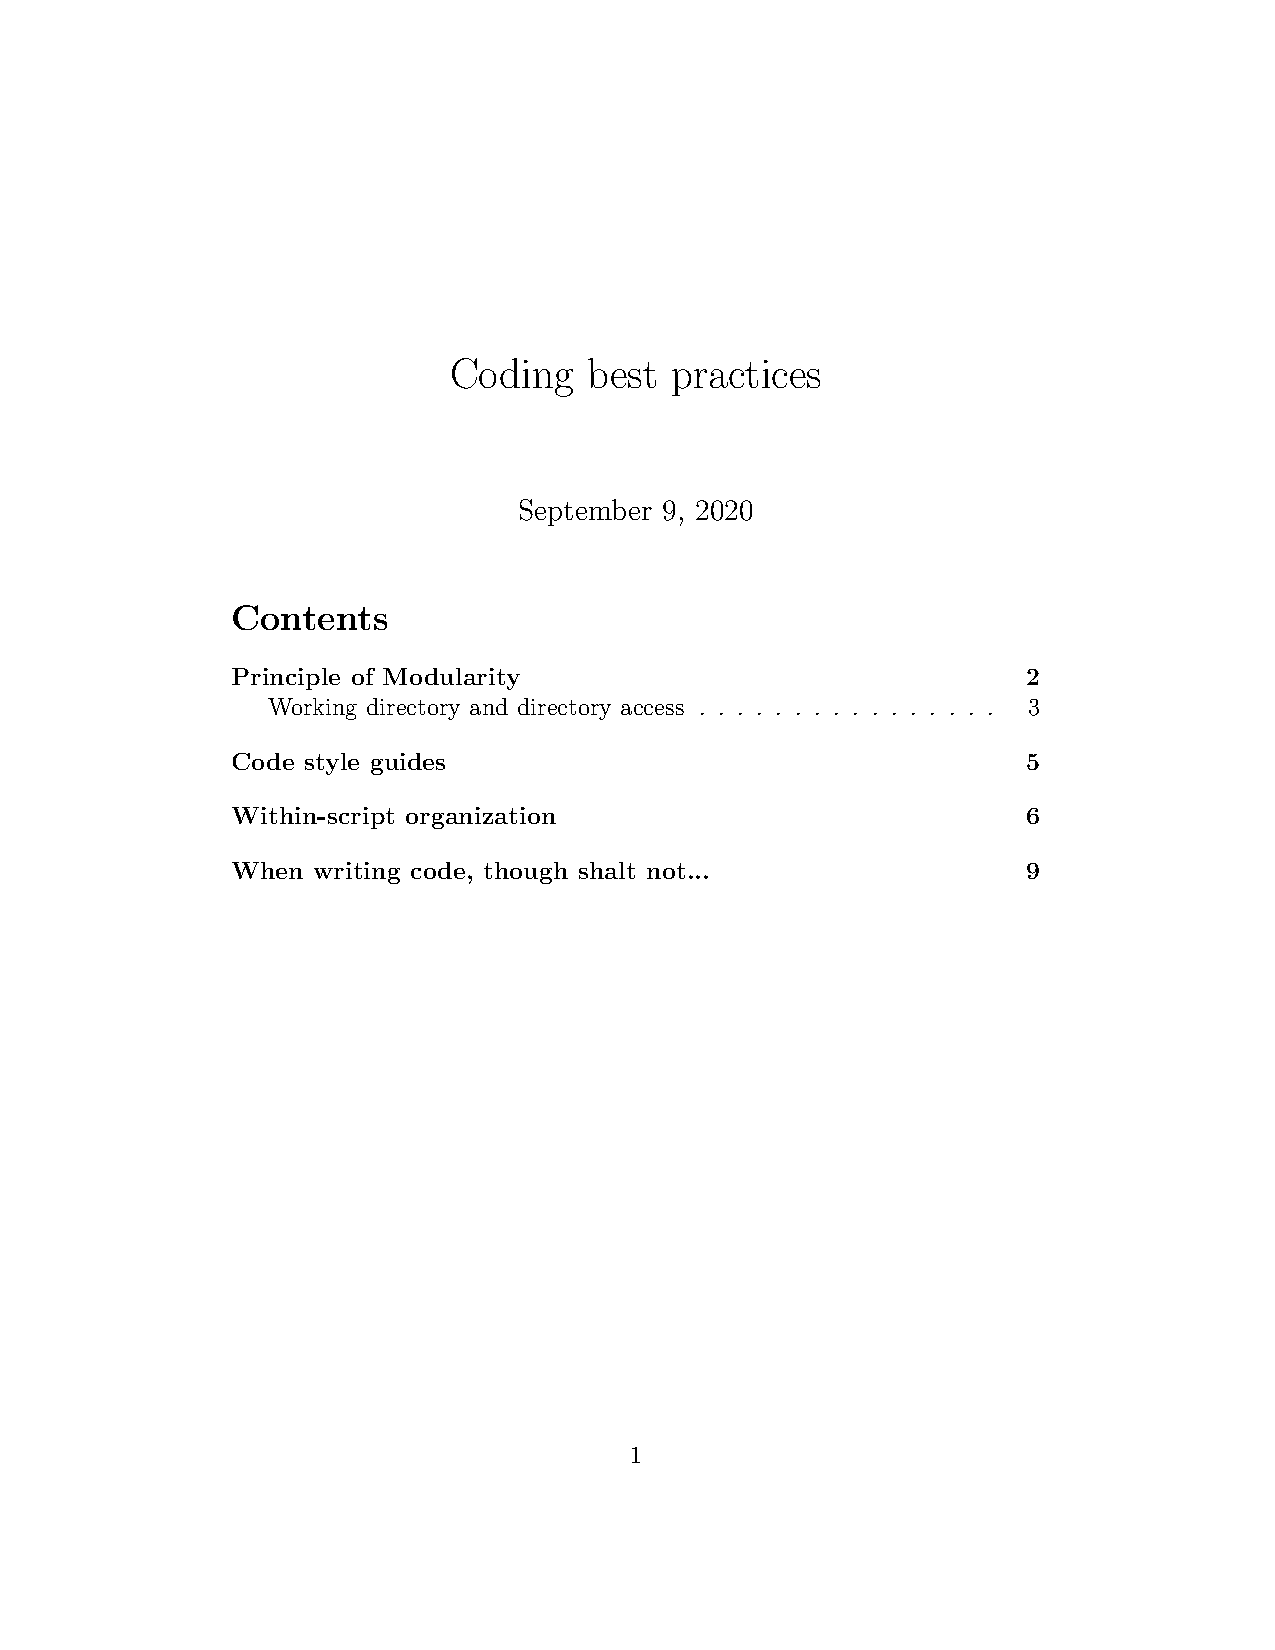
\includepdf[pages=-]{../../classes/CodingBestPractices/tex/CodingBestPractices.pdf}
	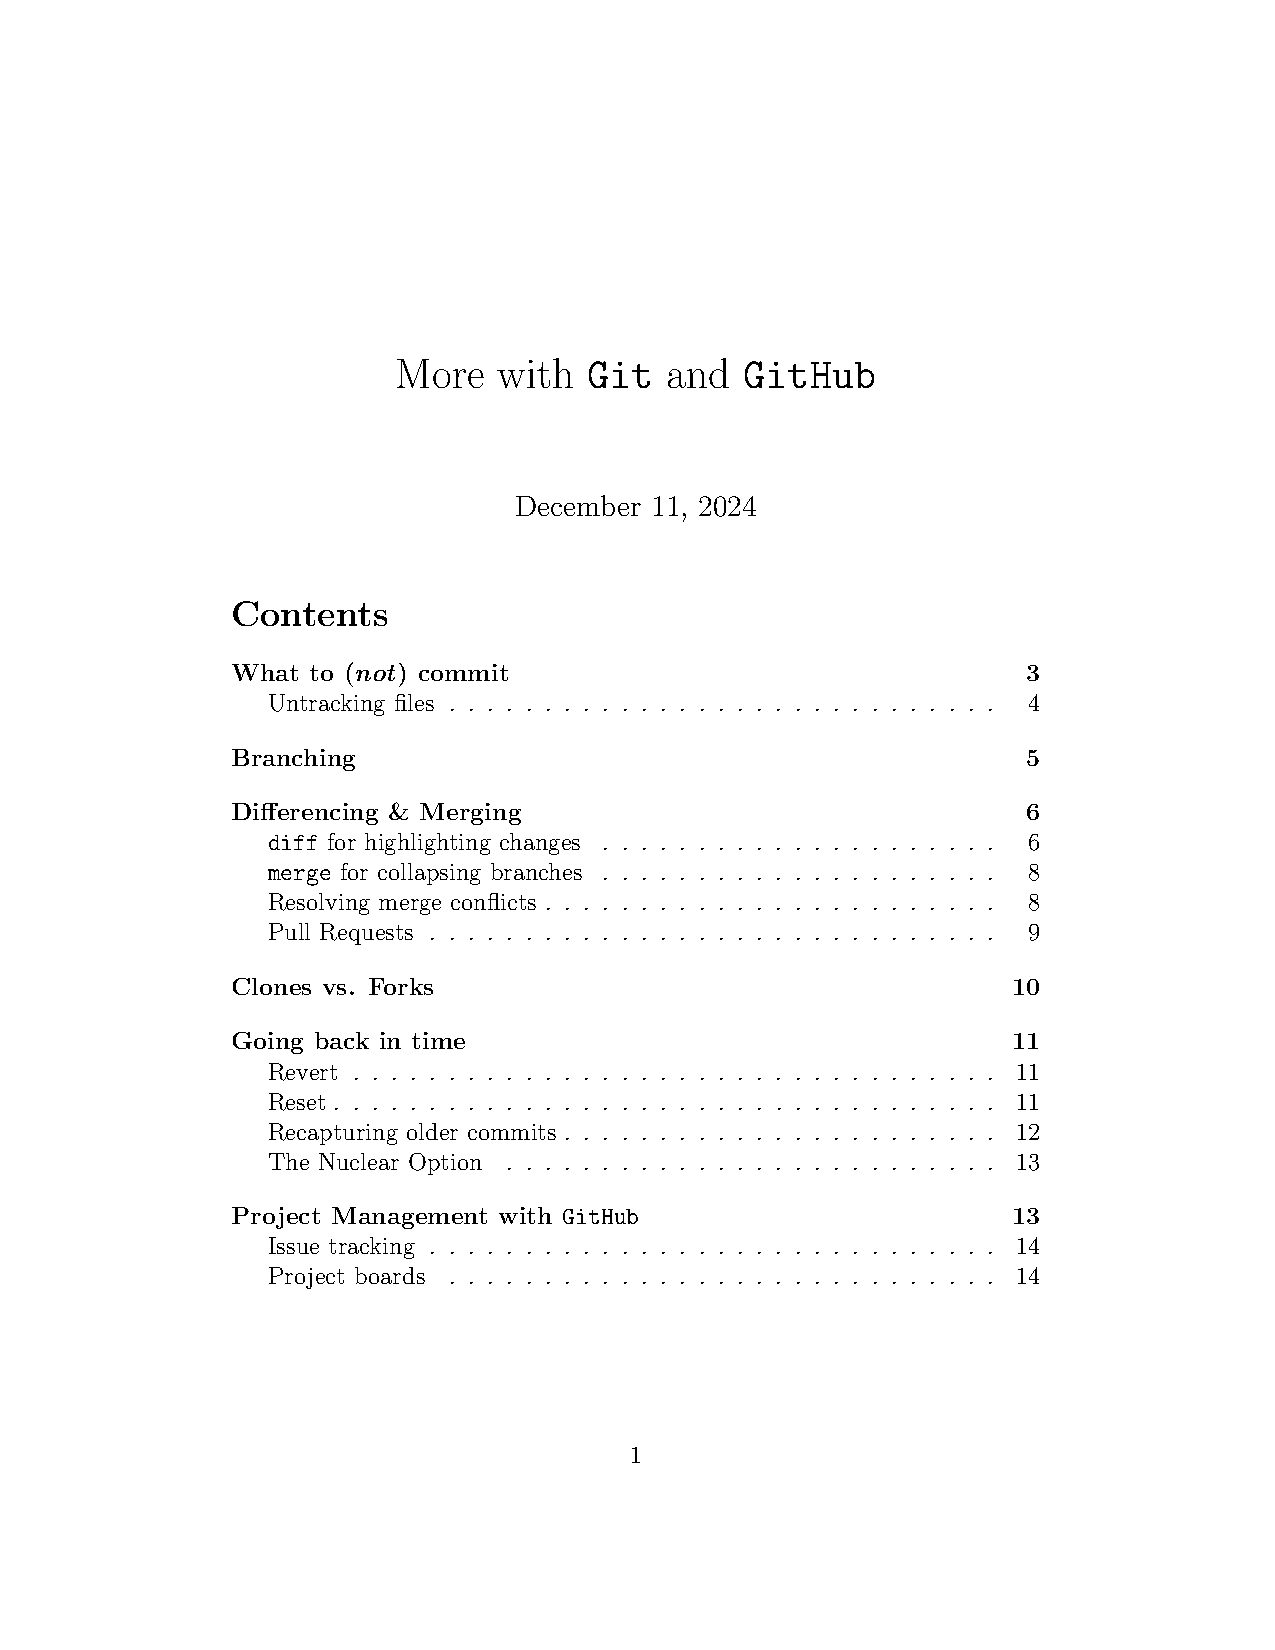
\includepdf[pages=-]{../../classes/VersionControl_Git_part_2/tex/Git_Part2.pdf}
	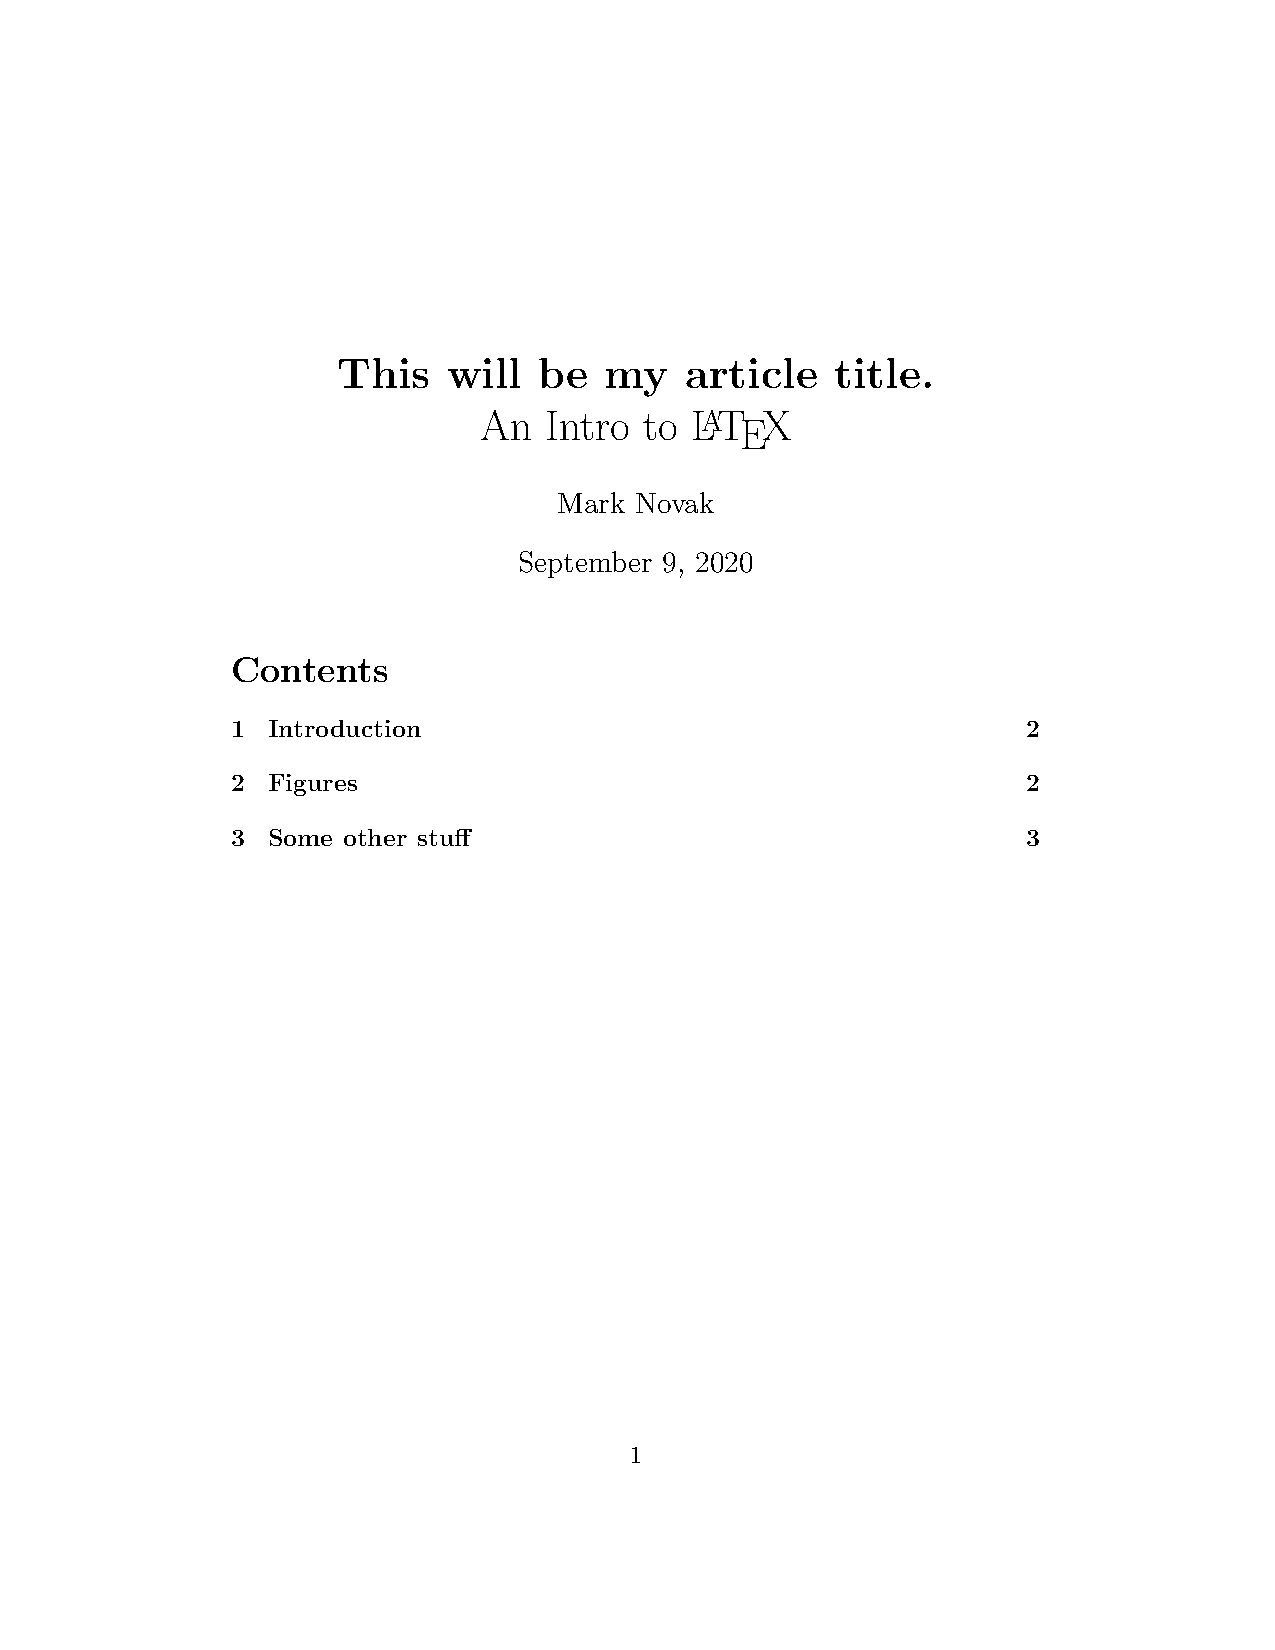
\includepdf[pages=-]{../../classes/Typesetting_LaTeX/tex/Intro2Latex.pdf}
	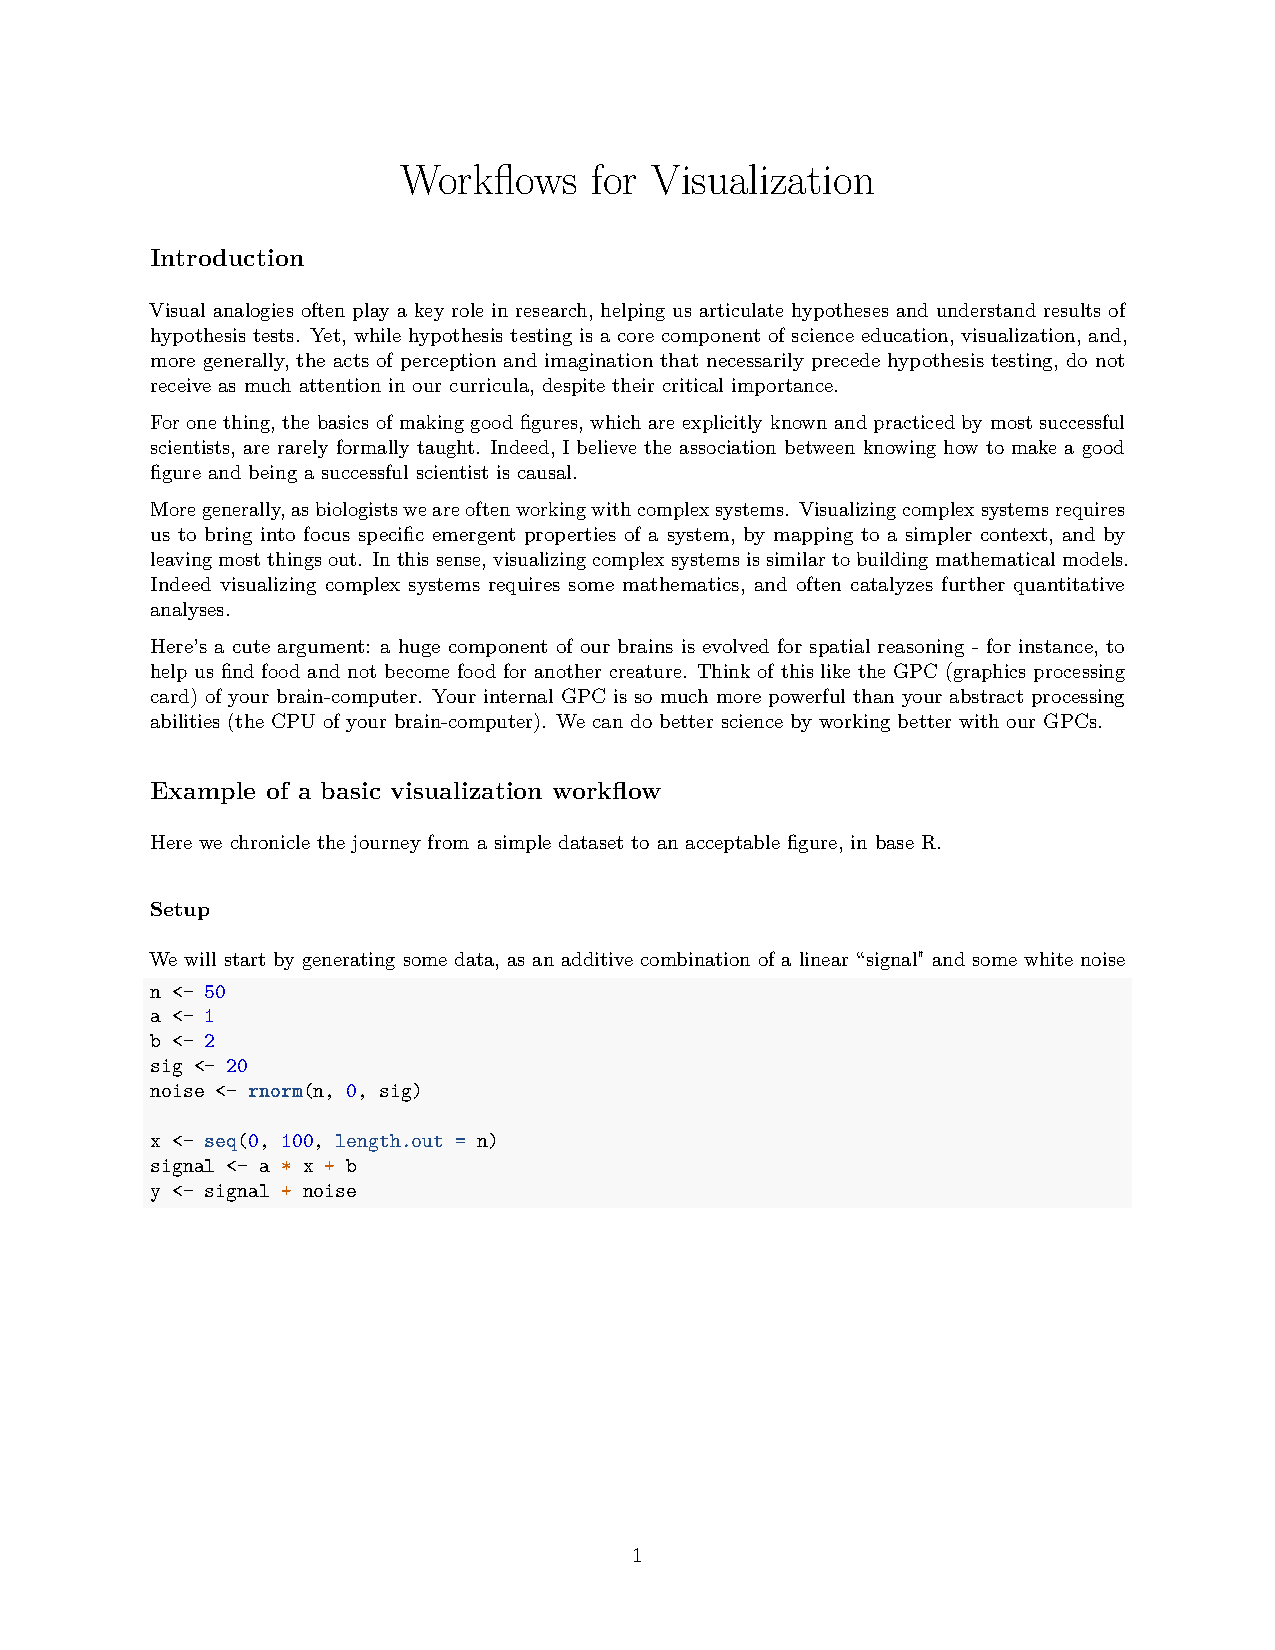
\includepdf[pages=-]{../../classes/Visualization/Rmd/visualization_part_1.pdf}

\end{document}
